\documentclass[ngerman
  ,numbers=noenddot % obsolete
  ,headsepline
  ,parskip=half*
  ,openany
  ,DIV=12
  ,fleqn % mv align to left
]{scrbook}
  %,12pt
  %,titelpage % unused
  %,biblography=totoc  % unused
  %,landscape,twocolumn
\usepackage[ngerman]{babel}
\usepackage[T1]{fontenc}
\usepackage[utf8]{inputenc}
%\usepackage[ansinew]{inputenc}
\usepackage{lmodern} %Type1-Schriftart für nicht-englische Texte

\setlength{\unitlength}{1mm}
\emergencystretch 2em

\usepackage{lscape} % alt: pdflscape
\usepackage{amsmath,amsthm,amssymb}
\usepackage{latexsym}
\usepackage{enumerate}
\usepackage{verbatim}
\usepackage{graphicx}

\allowdisplaybreaks

%\usepackage{thmbox}

%\usepackage{natbib}

\usepackage[automark]{scrpage2} % Headline styles
\usepackage[square,numbers]{natbib}


\pagestyle{scrheadings}
%A better solution would be to use typearea package.


% Section Numbers moved left out
%\usepackage{sectsty}
%\makeatletter\def\@seccntformat#1{%
  %\protect\makebox[0pt][r]{\csname the#1\endcsname\hspace{12pt}}}\makeatother

% semibold instead of bold
%\renewcommand{\bfdefault}{sb}

\renewcommand*{\thefootnote}{[\arabic{footnote}]}

% Zeichen
\usepackage{nicefrac}
\usepackage{mathrsfs}
\usepackage{stmaryrd}
%simplewick

\usepackage{tikz}
\usetikzlibrary{matrix,arrows,decorations.pathmorphing}

\numberwithin{equation}{chapter}
\numberwithin{figure}{chapter}

%%%%  Abkürzungsverzeichnis  %%%%%%%%%%%%%%%%%%%%%%%%%%%%%%%%%%%%%%%%
\usepackage{nomencl}
% Befehl umbenennen in abk
\let\abk\nomenclature
% Deutsche Überschrift
\renewcommand{\nomname}{Abkürzungsverzeichnis}
% Punkte zw. Abkürzung und Erklärung
\setlength{\nomlabelwidth}{.20\hsize}
\renewcommand{\nomlabel}[1]{#1 \dotfill}
% Zeilenabstände verkleinern
\setlength{\nomitemsep}{-\parsep}
\makenomenclature

%% BASH: makeindex main.nlo -s nomencl.ist -o main.nls

%%%%  Theoreme Styles  %%%%%%%%%%%%%%%%%%%%%%%%%%%%%%%%%%%%%%%%%%%%%%
\makeatletter

\theoremstyle{plain}% default
\newtheorem{thm}{Satz}[chapter]
%\newtheorem{thm}[satz]{Satz}
\newtheorem{lemma}[thm]{Lemma}
\newtheorem{lem}[thm]{Lemma}
\newtheorem{kor}[thm]{Korollar}
\newtheorem{prop}[thm]{Proposition}
\newtheorem{cor}[thm]{Korollar}

\theoremstyle{definition}
\newtheorem{defn}[thm]{Definition}
\newtheorem{conj}[thm]{Conjecture}
\newtheorem{exmp}[thm]{Beispiel}

\theoremstyle{remark}
\newtheorem{rem}[thm]{Bemerkung}
\newtheorem{bem}[thm]{Bemerkung}
\newtheorem{note}[thm]{Notiz}
\newtheorem{case}{Fall}

%custom pdf-metadata
%\pdfinfo{
%/Title (Title)
%/Subject (Subject)
%/Author (Maximilian Huber)
%/Keywords (keywords) }

\usepackage[german]{varioref}
%\usepackage[nameinlink,german]{cleveref}
\usepackage[colorlinks=true,linkcolor=black]{hyperref}

%% Autoref Names %%%%%%%%%%%%%%%%%
%\crefname{lemma}{Lemma}{Lemmas}
%\crefname{equation}{Gleichung}{Gleichungen}
%\crefname{definition}{Definition}{Definitionen}
%\crefname{algorithmus}{Algorithmus}{Algorithmen}
%\crefname{kor}{Korollar}{Korollare}

%%%%  new Commands  %%%%%%%%%%%%%%%%%%%%%%%%%%%%%%%%%%%%%%%%%%%%%%%%%
\def\bme{\boldsymbol{e}}

\def\A{\ensuremath \mathbb{A}}
%\def\B{\ensuremath \mathbb{B}}
\def\C{\ensuremath \mathbb{C}}
%\def\D{\ensuremath \mathbb{D}}
%\def\E{\ensuremath \mathbb{E}}
%\def\F{\ensuremath \mathbb{F}}
%\def\G{\ensuremath \mathbb{G}}
%\def\H{\ensuremath \mathbb{H}}
\def\I{\ensuremath \mathbb{I}}
%\def\J{\ensuremath \mathbb{J}}
%\def\K{\ensuremath \mathbb{K}}
%\def\L{\ensuremath \mathbb{L}}
%\def\M{\ensuremath \mathbb{M}}
\def\N{\ensuremath \mathbb{N}}
%\def\O{\ensuremath \mathbb{O}}
%\def\P{\ensuremath \mathbb{P}}
%\def\Q{\ensuremath \mathbb{Q}}
\def\R{\ensuremath \mathbb{R}}
%\def\S{\ensuremath \mathbb{S}}
%\def\T{\ensuremath \mathbb{T}}
%\def\U{\ensuremath \mathbb{U}}
%\def\V{\ensuremath \mathbb{V}}
%\def\W{\ensuremath \mathbb{W}}
%\def\X{\ensuremath \mathbb{X}}
%\def\Y{\ensuremath \mathbb{Y}}
\def\Z{\ensuremath \mathbb{Z}}

%\def\cA{\ensuremath \mathcal{A}}
%\def\cB{\ensuremath \mathcal{B}}
\def\cC{\ensuremath \mathcal{C}}
\def\cD{\ensuremath \mathcal{D}}
%\def\cE{\ensuremath \mathcal{E}}
%\def\cF{\ensuremath \mathcal{F}}
%\def\cG{\ensuremath \mathcal{G}}
%\def\cH{\ensuremath \mathcal{H}}
%\def\cI{\ensuremath \mathcal{I}}
%\def\cJ{\ensuremath \mathcal{J}}
%\def\cK{\ensuremath \mathcal{K}}
%\def\cL{\ensuremath \mathcal{L}}
\def\cM{\ensuremath \mathcal{M}}
\def\cN{\ensuremath \mathcal{N}}
%\def\cO{\ensuremath \mathcal{O}}
\def\cP{\ensuremath \mathcal{P}}
%\def\cQ{\ensuremath \mathcal{Q}}
%\def\cR{\ensuremath \mathcal{R}}
%\def\cS{\ensuremath \mathcal{S}}
%\def\cT{\ensuremath \mathcal{T}}
%\def\cU{\ensuremath \mathcal{U}}
%\def\cV{\ensuremath \mathcal{V}}
%\def\cW{\ensuremath \mathcal{W}}
%\def\cX{\ensuremath \mathcal{X}}
%\def\cY{\ensuremath \mathcal{Y}}
%\def\cZ{\ensuremath \mathcal{Z}}

%\def\sA{\ensuremath \mathscr{A}}
%\def\sB{\ensuremath \mathscr{B}}
%\def\sC{\ensuremath \mathscr{C}}
%\def\sD{\ensuremath \mathscr{D}}
\def\sE{\ensuremath \mathscr{E}}
%\def\sF{\ensuremath \mathscr{F}}
%\def\sG{\ensuremath \mathscr{G}}
%\def\sH{\ensuremath \mathscr{H}}
%\def\sI{\ensuremath \mathscr{I}}
%\def\sJ{\ensuremath \mathscr{J}}
%\def\sK{\ensuremath \mathscr{K}}
%\def\sL{\ensuremath \mathscr{L}}
%\def\sM{\ensuremath \mathscr{M}}
%\def\sN{\ensuremath \mathscr{N}}
%\def\sO{\ensuremath \mathscr{O}}
%\def\sP{\ensuremath \mathscr{P}}
%\def\sQ{\ensuremath \mathscr{Q}}
%\def\sR{\ensuremath \mathscr{R}}
%\def\sS{\ensuremath \mathscr{S}}
%\def\sT{\ensuremath \mathscr{T}}
%\def\sU{\ensuremath \mathscr{U}}
%\def\sV{\ensuremath \mathscr{V}}
%\def\sW{\ensuremath \mathscr{W}}
%\def\sX{\ensuremath \mathscr{X}}
%\def\sY{\ensuremath \mathscr{Y}}
%\def\sZ{\ensuremath \mathscr{Z}}

%\renewcommand{\headrulewidth}{0.2pt}

\newcommand{\myhr}{\rule{0.3\textwidth}{1pt}}

\let\epsilon\varepsilon
\let\phi\varphi

\DeclareMathOperator{\modulo}{mod}
\DeclareMathOperator{\conv}{conv}
\DeclareMathOperator{\Cof}{Cof}
\DeclareMathOperator{\grad}{grad}
\DeclareMathOperator{\Id}{Id}
\DeclareMathOperator{\dist}{dist}
\DeclareMathOperator{\diam}{diam}
\DeclareMathOperator{\co}{co}
\DeclareMathOperator{\supp}{supp}
\DeclareMathOperator{\graph}{graph}
\DeclareMathOperator{\slopes}{slopes}
\DeclareMathOperator{\Ob}{Ob}
\DeclareMathOperator{\Mor}{Mor}

% specific:
\newcommand{\Dm}{{\cD\mbox{-Modul}}}

\newcommand{\Cfx}{{\mathbb C\llbracket x\rrbracket}}
\newcommand{\Cft}{{\mathbb C\llbracket t\rrbracket}}
\newcommand{\Cfu}{{\mathbb C\llbracket u\rrbracket}}
\newcommand{\Ckx}{{\mathbb C (\!(x)\!)}}
\newcommand{\Ckt}{{\mathbb C (\!(t)\!)}}
\newcommand{\Cku}{{\mathbb C (\!(u)\!)}}

\makeatother

\newcommand{\overbox}[2]{\ensuremath\begin{array}[b]{c}%
\makebox[0pt]{\fbox{\scriptsize#2}}\\[-2pt]\text{\small$\downarrow$}\\[-3pt]%
{\displaystyle#1}\end{array}}%


\usepackage{xcolor}
\usepackage{color}
\usepackage{framed}

\newenvironment{fshaded}{%
\def\FrameCommand{\fcolorbox{framecolor}{shadecolor}}%
\MakeFramed {\FrameRestore}}%
{\endMakeFramed}

%\newenvironment{comment}{\definecolor{shadecolor}{rgb}{1,.6,.6}%
%\definecolor{framecolor}{rgb}{0,0,0}%
%\begin{fshaded}}{\end{fshaded}}

\renewcommand{\comment}{\definecolor{shadecolor}{rgb}{.8,.8,.8}%
\definecolor{framecolor}{rgb}{0,0,0}%
\fshaded}
\renewcommand{\endcomment}{\endfshaded}

%Zeilenhöhe, für bessere lesbarkeit
\linespread{1.3}

\cfoot{-\thepage-\\\today}
\setboolean{@twoside}{false} 

%\usepackage{showframe}


\begin{document}

%TODO: set titel variable??

%%%%%%%%%%%%%%%%%%%%%%%%%%%%%%%%%%%%%%%%%%%%%%%%%%%%%%%%%%%%%%%%%%%%%
\frontmatter

\begin{titlepage}
  \thispagestyle{empty}
  \newcommand{\Rule}{\rule{\textwidth}{1mm}}
  \begin{center}\sffamily\bfseries
    \LARGE Bachelorarbeit
    \vfill
    \Rule\vspace{5mm}
    \Huge
    mein thema
    \vspace{1mm}\Rule
    \vfill
    \normalfont\sffamily\large vorgelegt von\par
    \bfseries\LARGE Maximilian Huber
    \vfill
    \normalfont\sffamily\large am\\
    \bfseries\Large Institut für Mathematik\\
    \normalfont\sffamily\large der\\
    \bfseries\Large Universität Augsburg
    \vfill
    \normalfont\sffamily\large betreut durch \\
    \bfseries\Large Prof. Dr. Marco Hien \par
    \vfill
    \normalfont\sffamily\large abgegeben am \\
    \bfseries\Large noch nicht\\
    stand: \today
  \end{center}
\end{titlepage}
% vim: set ft=tex :


%\begin{center}
  %\today
%\end{center}
\tableofcontents{}
%\printnomenclature

%\newpage

\chapter{Einleitung}


\mainmatter
%%%%%%%%%%%%%%%%%%%%%%%%%%%%%%%%%%%%%%%%%%%%%%%%%%%%%%%%%%%%%%%%%%%%%
\part{Theorie}

\chapter{Mathematische Grundlagen}

Hier werde ich mich auf \cite{sabbah_cimpa90} und \cite{coutinho1995primer} beziehen.

\section{Einige Ergebnise aus der Kommutativen Algebra}~

In dieser Arbeit spielen die folgenden Ringe eine Große Rolle:
\begin{itemize}
  \item $\C[x]:=\{ \sum^{N}_{i=1}a_ix^i | N\in \N \}$
  \item $\C\llbracket x\rrbracket:=\{ \sum^{\infty}_{i=1}a_ix^i \}$
  \item $\C\{x\}:=\{ \sum^{\infty}_{i=1}a_ix^i | \mbox{pos.
        Konvergenzradius} \}$
  \item $K:=\C(\{x\}):=\C\{x\}[x^{-1}]$
  \item $\hat{K}:=\C((x)):=\C\llbracket x\rrbracket[x^{-1}]$
\end{itemize}

wobei offensichtlich gilt $\C[x]\subset\C\{x\}\subset\C\llbracket x\rrbracket$.

\begin{comment}
  \begin{lem}[Seite 2]
    ein paar eigenschaften
    \begin{enumerate}
      \item $\C[x]$ ist ein graduierter Ring, durch die Grad der
        Polynome. Diese graduierung induziert eine aufsteigende Filtrierung.

        alle Ideale haben die form $(x-a)$ mit $,a\in \C$
      \item wenn $\mathfrak{m}$ das maximale Ideal von $\C[x]$ (erzeugt von
        $x$ ist), so ist
        \[
          \C[[x]]=
          \underset{k}{\underleftarrow{\lim}} \C[X]\backslash\mathfrak{m}^k
        \]
        The ring $\C[[x]]$ ist ein nöterscher lokaler Ring:
        jede Potenzreihe mit konstantem term $\neq0$ ist invertierbar.

        Der ring ist ebenfalls ein diskreter ??? Ring (discrete valuation
        ring)

        Die Filtrierung nach grad des Maximalen Ideals, genannt
        $\mathfrak{m}$-adische Fitration, ist die Filtrierung
        $\mathfrak{m}^k=\{f\in \C[[x]]|v(f)\geq k\}$

        und es gilt $gr_\mathfrak{m}(\C[[x]])=\C[x]$
      \item $\C\{x\}\subset \C[[x]]$ ist ein Untering der Potenzreihen, wobei
        der Konvergenzradius echt positiv ist.

        ist ähnlich zu $\C[[x]]$
    \end{enumerate}
  \end{lem}
\end{comment}

\begin{defn}[Kommutator]%zula seite 15
  Sei $R$ ein Ring. Für $a,b\in R$ wird
  \[[a,b]=b\cdot a-a\cdot b\]
  der \emph{Kommutator von a und b} genannt.
\end{defn}

\section{Weiterführende Definitionen}~

\begin{defn}[pull-back]
  Der \emph{pull-back} $\rho^{+}M$ ist der Vektorraum
  $\rho^{*}M=\C((u))\otimes_{\C((u))}M$ mit
  der \emph{pull-back Verknüpfung(connection)} $\rho^*\nabla$ definiert durch
  $\partial_u(1\otimes m):=\rho'(u)\otimes\partial_tm$
\end{defn}

sei nun $N$ ein $\C((u))$-VR mit Verknüpfung
\begin{defn}[push-forward]
  Der \emph{push-forward} $\rho_+N$ ist definiert durch:
  \begin{itemize}
    \item der $\C((t))$-VR $\rho_*N$ ist der $\C$-VR N mit der $\C((t))$
      Struktur durch $f(t)\cdot 0:=f(\rho(t))m$
    \item die wirkung von $\partial_t$ ist die von $\rho'(u)^-1\partial_u$
  \end{itemize}
\end{defn}
\begin{thm} \label{thm:Projektionsformel}
  es gilt dir Projektionsformel
  \begin{equation} \label{eq:Projektionsformel}
    \rho_+(N\otimes_{\C((u))}\rho^+M)\cong\rho_+N\otimes_{\C((t))}M
  \end{equation}
\end{thm}

\begin{comment}
  TEST für ref\\
  \ref{thm:Projektionsformel}\\
  TEST für eqref\\
  \eqref{eq:Projektionsformel}\\
\end{comment}

\section{Weyl-Algebra und der Ring $\D$} %TODO: sabah-cimpa90.pdf  seite 3
Ich werde hier die Weyl Algebra, wie in
\cite[Chapter~1]{sabbah_cimpa90}, in einer Veränderlichen einführen.
Sei $\frac{\partial}{\partial x}=\partial_x$ der Ableitungsoperator nach $x$
und sei f $\in\C[x]$ (bzw. $\C\{x\}$ bzw. $\C\llbracket x\rrbracket$).
Man hat die folgende Kommutations-Relation zwischen dem
\emph{Ableitungsoperator}
und dem \emph{Multiplikations Operator} f:
\begin{equation}\label{eq:weyl_relation}
  [\frac{\partial}{\partial x},f]=\frac{\partial f}{\partial x}
\end{equation}
wobei die Rechte Seite die Multiplikation mit $\frac{\partial f}{\partial x}$
darstellt. Dies bedeutet für alle $g\in\C[x]$ hat man:
\[
  [\frac{\partial}{\partial x},f]\cdot g
  =\frac{\partial fg}{\partial x} - f\frac{\partial g}{\partial x}
  =\frac{\partial f}{\partial x} \cdot g
\]
\begin{defn}[Weyl Algebra]
  Definiere nun die Weyl Algebra $A_1(\C)$ (bzw. die Algebra $\D$ von
  linearen Operatoren mit Koeffizienten in $\C\{x\}$ bzw. die Algebra
  $\hat{\D}$ (Koeffizienten in $\C\llbracket x\rrbracket$)) als die
  Quotientenalgebra der freien Algebra, welche von dem Koeffizientenring
  zusammen mit dem Element $\partial_x$, erzeugt wird, Modulo der Relation
  \eqref{eq:weyl_relation}.
\end{defn}
Wir werden die Notation $A_1(\C)=\C[x]<\partial_x>$ (bzw.
$\D=\C\{x\}<\partial_x>$ bzw. $\hat{\D}=\C[[x]]<\partial_x>$) verwenden.

\begin{comment}
  \textbf{countinho's ansicht:}
  Sei $K\{z_1,...,z_{2n}\}$ eine freie Algebra in $2n$ variablen. Die
  Multiplikation von zwei Monomen ist als einfaches Nebeneinanderschreiben
  Definiert. Betrachte nun den folgenden Homomorphismus:
  \[ \phi:K\{z_1,...,z_{2n}\}\rightarrow A_n \]
  mit $\phi(z_i)=x_i$ und $\phi(z_{i+n})=\partial_i$ für $i\in\{1,..,n\}$.\\
  Sei $J$ das (two sided) Ideal von $K\{x_1,..,x_{2n}\}$ generiert durch:
  \begin{itemize}
    \item $[z_{i+n},z_i]-1$ für $i=1,...,n$
    \item $[z_i,z_j]$
      für $j\neq i+n$ und $1\leq i,j\leq 2n$
  \end{itemize}
  So dass $\phi$ einen homomorphismus
  \[ \phi:K\{z_1,...,z_{2n}\}/J\rightarrow A_n \]
  induziert.

\end{comment}

\begin{rem}
  $A_1(\C),~\D$ und $\hat\D$ sind nicht kommutative Algebren.
\end{rem}

\begin{lem}
  Es gelten die Formeln\\
  %\begin{eqnarray*}
    %[\partial_x,x^k] & = & kx^{k-1}\\
    %[\partial_x^j,x] & = & j\partial_x^{j-1}\\
    %[\partial_x^j,x^k] & = & \sum_{i\geq1}\frac{}{}x^{k-i}\partial_x^{j-i}\\
  %\end{eqnarray*}
  $ [\partial_x,x^k] = kx^{k-1} $\\
  $ [\partial_x^j,x] = j\partial_x^{j-1} $\\
  $ [\partial_x^j,x^k] = \sum_{i\geq1}\frac{k(k-1)\cdots(k-i+1)
    \cdot j(j-1)\cdots(j-i+1)}{i!}x^{k-i}\partial_x^{j-i} $
\end{lem}
\begin{proof}
  Zula Barbara
\end{proof}

\begin{prop} \label{prop:weyl_eindeutige_schreibung}
  Jedes Element in $A_1(\C)$ (bzw. $\D$ oder $\hat{\D}$) kann auf eindeutige
  weiße als $P=\sum_{i=0}^na_i(x)\partial_x^i$, mit $a_i(x)\in A_1(\C)$ (bzw.
  $\D$ oder $\hat{\D}$), geschrieben werden. 
\end{prop}
\begin{proof}
  \cite[Proposition 1.2.3]{sabbah_cimpa90}
  \begin{comment}
    ein teil des Beweises ist "left as an exersice"
  \end{comment}
\end{proof}

%TODO: definition Filtrierung und Grad 

\begin{defn}
  Sei $\deg P=\sum_{i=0}^na_i(x)\partial_x^i$ bzgl. $n$ minimal geschrieben, so 
  ist $\deg P:=n$ der \emph{Grad von $P$}. So definiere 
  $F_N\D:=\{P\in\D|\deg P\leq N\}$ und erhalte die aufsteigende Filtrierung
  \[
    \cdots\subset F_{-1}\D\subset F_{0}\D\subset F_{1}\D\subset\cdots\subset\D
  \]
  und erhalte $gr_k^F\D\underset{\mbox{def}}{=}F_N\D\slash F_{N-1}\D
  =\{P\in\D|\deg P=N\}\cong\C\{x\}$.
\end{defn}

\begin{proof}
  \begin{comment}
    mit isom: $[P]=P+F_{N-1}\D\mapsto a_n(x)$
  \end{comment}
\end{proof}

\begin{prop}
  Es gilt:
  \begin{center}
    \begin{tikzpicture} [descr/.style={fill=white,inner sep=2.5pt}]
    \matrix (m) [
      matrix of math nodes,
      row sep=1em,
      %column sep=-0.7em,
      text height=1.5ex,
      text depth=0.25ex]
    {
      gr^F\D &
      := &
      \bigoplus_{\N\in\Z}gr_N^F\D &
      = &
      \bigoplus_{\N\in\N_0}gr_N^F\D &
      \cong &
      \bigoplus_{\N\in\N_0}\C\{x\} &
      \cong &
      \C\{x\}[\xi] &
      = &
      \bigoplus_{\N\in\N_0}\C\{x\}\cdot \xi^N \\
    };
      \path[solid]
      (m-1-1) edge [bend right=20] node[descr]{$\cong$}
        node[below]{$\mbox{Isom. von grad. Ringen}$} (m-1-11);
    \end{tikzpicture}
  \end{center}
\end{prop}

\begin{comment}
  \subsection{Weyl Algebra als Graduierter Ring}
  % Treffen 2
  Sei $A$ nun einer der drei Koeffizienten Ringe, welche zuvor behandelt wurden.
  Der Ring $A<\partial_x>$ kommt zusammen mit einer aufsteigenden Filtrierung,
  welche wir mit $F(A<\partial_x)$ bezeichen werden.
  Sei $P$ ein bzgl. \ref{prop:weyl_eindeutige_schreibung} minimal geschriebener
  Operator, so ist $P$ in $F_k$ falls der maximale Grad von $\partial_x$ in $P$
  kleiner oder gleich $k$. So definiere den Grad $deg P$ von $P$ als die 
  Eindeutige ganze Zahl $k$ mit $P\in F_kA<\partial_x>\slash F_{k-1}<\partial_x>$
  \begin{comment}
    Unabhängigkeit von Schreibung wird in Sabbah Script behauptet
  \end{comment}
\end{comment}

\section{Struktur von Links-Idealen auf $\D$}

\section{Lokalisierung eines $\C\{x\}$-Modules} %TODO: Modules or Moduls

\section{Lokalisierung eines holonomen $\D$-Modules}

% vim: set ft=tex :

%\newpage

% In chapter "Meromorphe Zusammenhänge" verschoben
%% das gleiche wie Meromorphe zusammenhänge?

\section{\cD-Moduln}

\subsection{Lokalisierung eines $\C\{x\}$-Moduls}

\begin{defn}
  Sei $M$ ein $\C\{x\}$-Modul und $K=\C\{x\}[x^{-1}]$, dann ist die
  Lokalisierung
  \[ M[x^{-1}]:=M\otimes_{\C\{x\}}K \,. \]
\end{defn}

\subsection{Lokalisierung eines holonomen $\cD$-Moduls}

%vim: set ft=tex :

%\newpage

% TODO; wie darf ich einen Meromorphen verändern, (das P verändern) ohne das
  % sich effektiv was ändert?
% TODO: \cM = \cM_K ... replace

\chapter{Der Meromorpher Zusammenhang}
Quelle ist \cite{sabbah_cimpa90}
\section{Definition}~

\begin{defn}[Meromorpher Zusammenhang]
  Ein (\emph{Keim eines}) \emph{Meromorpher Zusammenhang} (an $x=0$)
  $(\cM_K,\partial)$ besteht aus folgenden Daten:
  \begin{itemize}
    \item $\cM_K$, ein endlich dimensionaler $K$-Vr
    \item einer $\C$-linearen Abbildung $\partial:\cM_K\rightarrow \cM_K$, genannt
      \emph{Derivation}, welche für alle $f\in K$ und $u\in \cM_K$ die
      \emph{Leibnitzregel}
      \begin{equation}\label{eq:Leibnitzregel}
        \partial(fu)=f'u+f\partial u
      \end{equation}
      erfüllen soll.
  \end{itemize}
\end{defn}

% hier gleich definition für formale meromorphe Zusammenhänge??

\begin{bem}
  Später wird man auf die Angabe von $\partial$ verichten und einfach $\cM_K$ als
  den Meromorphen Zusammenhang bezeichnen.
\end{bem}

\section{Eigenschaften}
Hier nun einige Eigenschaften Meromorpher Zusammenhänge.

\begin{lem}
  Sei $\cM_K$ ein Meromorpher Zusammenhang, dann existiert ein $P\in??$ so dass
  $\cM_K\cong\cD/\cD\cdot P$.
\end{lem}

\begin{lem}
  %TODO: hier $\cM ??
  Sei $(\cM_K,\partial)$ ein gegebener Meromorpher Zusammenhang, und $\phi$ ein
  Basisisomorphismus von $K^r$ nach $\cM_K$, also in der Situation
  \begin{center}
    \begin{tikzpicture} [scale=3.3, descr/.style={fill=white,inner sep=2.5pt} ]
    \matrix (m) [
      matrix of math nodes
      , row sep=3em
      , column sep=3em
      %, text height=3em
      %, text depth=0.25em
      ]
    {
      \cM_K & \cM_K \\
      K^r & K^r \\
    };
      \path[->,font=\scriptsize,>=angle 90]
      (m-1-1) edge node[above]{$\partial$} (m-1-2)
      (m-2-1) edge node[above]{$\phi^{-1}\partial\phi$} (m-2-2)
      ;
      %TODO: make this harpoon arrows
      \path[->,font=\scriptsize,>=angle 90]
      (m-2-1) edge node[descr]{$\cong$} node[right]{$\phi$} (m-1-1)
      (m-2-2) edge node[descr]{$\cong$} node[left]{$\phi$} (m-1-2)
      ;

      \path[>=stealth,|->]
      ;
    \end{tikzpicture}
  \end{center}
  gilt: $(K^r,\phi^{-1}\partial\phi)$ ist ebenfalls ein Meromorpher Zusammenhang.
\end{lem}
\begin{proof}
  TODO, (3. Treffen)
\end{proof}

Sind $\partial_1$ und $\partial_2$ zwei Meromorphe Zusammenhänge auf $\cM_K\cong
K^r$. So betrachte $\partial_1-\partial_2:\cM\rightarrow\cM$ für alle $f\in K$ 
und $u\in \cM_K$ :
\begin{align*}
  (\partial_1-\partial_2)(fu) &= \partial_1(fu)-\partial_2(fu)\\
  &= f'u+f\partial_1u-f'u-f\partial_2u\\
  &= f\cdot(\partial_1-\partial_2)(u)\\
\end{align*}
\begin{lem}
  Da $\partial_1-\partial_2$ $\C$-linear und, wie eben gezeigt,
  $(\partial_1-\partial_2)(fu)=f\cdot(\partial_1-\partial_2)(u)$ allgemein
  gilt: Die differenz zweier Meromorpher Zusammenhäge ist $K$-linear.
  %Differenz zweier Meromorpher Zshg. ist K-linear
\end{lem}
Insbesondere ist $\frac{d}{dz}-\partial:K^r\rightarrow K^r$ $K$-linear, also es
existiert eine Matrix $A\in M(r\times r,K)$ mit $\frac{d}{dz}-\partial=A$, also
ist $\partial=\frac{d}{dz}-A$.

%TODO: beobachtung...

%TODO: differenz ist linear

\begin{defn}[Transformationsformel]
  In der Situation

  \begin{center}
    \begin{tikzpicture} [scale=3.3, descr/.style={fill=white,inner sep=2.5pt} ]
    \matrix (m) [
      matrix of math nodes
      , row sep=3em
      , column sep=3em
      %, text height=3em
      %, text depth=0.25em
      ]
    {
      K^r & & & K^r \\
       & M & M & \\
      K^r & & & K^r \\
    };
      \path[->,font=\scriptsize,>=angle 90]
      (m-1-1) edge node[descr]{$\cong$} node[above]{$\phi$} (m-2-2)
      (m-3-1) edge node[descr]{$\cong$} node[above]{$\psi$} (m-2-2)
      (m-1-4) edge node[descr]{$\cong$} node[above]{$\phi$} (m-2-3)
      (m-3-4) edge node[descr]{$\cong$} node[above]{$\psi$} (m-2-3)

      (m-2-2) edge node[above]{$\partial$} (m-2-3)

      (m-1-1) edge node[above]{$\frac{d}{dz}+A$} (m-1-4)
      (m-3-1) edge node[above]{$\frac{d}{dz}+B$} (m-3-4)

      (m-3-1) edge node[descr]{$\cong$} node[right]{$T$} (m-1-1)
      (m-3-4) edge node[descr]{$\cong$} node[left]{$T$} (m-1-4)
      ;

      \path[>=stealth,|->]
      ;
    \end{tikzpicture}
  \end{center}
  mit $\phi,\psi$ und $T$ $K$-Linear und $\partial,(\frac{d}{dz}+A)$ und
  $(\frac{d}{dz}+B)$ $\C$-Linear, gilt:\\
  Der Merom. Zush. $\frac{d}{dz}+A$ auf $K^r$ wird durch Basiswechsel $T\in
  GL(r,K)$ zu
  \[
    \frac{d}{dz}+(T^{-1}\cdot T'+T^{-1}AT) = \frac{d}{dz}+B
  \]
\end{defn}
\begin{defn}
  $A\sim B$ differenziell Äquivalent $:\Leftrightarrow$ $\exists T\in GL(r,K)$
  mit $B=T^{-1}\cdot T'+T^{-1}AT$
\end{defn}

\begin{comment}
  $1=TT^{-1}$ $\rightsquigarrow$ $T'T^{-1}+T(T^{-1})'=0$\\
  $1=T^{-1}T$ $\rightsquigarrow$ $(T^{-1})'T+T^{-1}T'=0$
\end{comment}

%TODO: titel: Operations on vector spaces with connection
\section{pull-back und push-forward}

nach \cite[1.a]{sabbah_Fourier-local}

\begin{defn}[pull-back]
  Der \emph{pull-back} $\rho^{+}\cM$ ist der Vektorraum
  $\rho^{*}\cM=\C((u))\otimes_{\C((u))}\cM$ mit dem \emph{pull-back
    Zusammenhang} $\rho^*\nabla$ definiert durch $\partial_u(1\otimes
  m):=\rho'(u)\otimes\partial_tm$
\end{defn}

sei nun $\cN$ ein weiterer $\C((u))$-VR mit Verknüpfung
\begin{defn}[push-forward]
  Der \emph{push-forward} $\rho_+\cN$ ist definiert durch:
  \begin{itemize}
    \item der $\C((t))$-VR $\rho_*\cN$ ist der $\C$-VR $\cN$ mit der $\C((t))$
      Struktur durch $f(t)\cdot m:=f(\rho(t))m$
    \item die wirkung von $\partial_t$ ist die von $\rho'(u)^{-1}\partial_u$
  \end{itemize}
\end{defn}
\begin{thm} \label{thm:Projektionsformel}
  es gilt dir Projektionsformel
  \begin{equation} \label{eq:Projektionsformel}
    \rho_+(\cN\otimes_{\C((u))}\rho^+\cM)\cong\rho_+\cN\otimes_{\C((t))}\cM
  \end{equation}
\end{thm}

\section{Formale Meromorphe Zusammenhänge}

\begin{defn}[Formaler Meromorpher Zusammenhang]
  Ein \emph{Formaler Meromorpher zusammenhang} $(\cM_{\hat{K}},\partial)$ besteht aus 
  folgenden Daten:
  \begin{itemize}
    \item $\cM_{\hat{K}}$, ein endlich dimensionaler $\hat K$-Vr
    \item eine \emph{Derivation} $\partial$, für die die \emph{Leibnitzregel} 
      \eqref{eq:Leibnitzregel}, für alle $f\in \hat K$ und $u\in \cM_{\hat K}$,
      erfüllt sein soll.
  \end{itemize}
\end{defn}

\begin{comment}
  Oder einfach ein Meromorpher Zshg. über anderes $K$ also $\hat K$
\end{comment}

\begin{bem}
  alle bisher gegebenen Definitionen und Lemmata gelten für formale Meromorphe
  Zusammenhänge analog wie für konvergente Meromorphe Zusammenhänge.
\end{bem}

\section{Elementare Meromorphe Zusammenhänge}

%TODO: auch nicht formal
\begin{defn}[Elementarer formaler Zusammenhang]
  Zu einem gegebenen $\rho\in u\C\llbracket u\rrbracket$, $\phi\in\C((u))$ und
  einem endlich dimensionalen $\C((u))$-Vektorraum $R$ mit regulärem 
  Zusammenhang $\nabla$, definieren wir den assoziierten Elementaren endlich
  dimensionalen $\C((t))$-Vektorraum mit Zusammenhang, durch:
  \[
    El(\rho,\phi,R)=\rho_+(\sE\otimes R)
  \]
\end{defn}

%TODO: weitere Eigenschaften

\section{Newton Polygon} % ist dies eine Invariante??
% gestohlen aus der ZulaBarbara Seite 46

Jedes $P\in \cD$ lässt sich eindeutig schreiben als
\[ P=\sum^{n}_{k=0}{\sum^{\infty}_{l=-N}{\alpha_{kl}t^l\partial_t^k}} \]
mit $\alpha_{kl}\in\C$ schreiben und betrachte das dazugehörige
\[ H:=\underset{k,l\mbox{ mit }\alpha_{kl}\neq0}{\bigcup}\{ (k,l-k) +
  \R_{\leq 0}\times \R_{\geq 0} \}\subset \R^2 \,. \]
\begin{comment}
  bei sabbah: $H\subset \N\times\Z$ und dann konvexe hülle davon in $\R^2$
\end{comment}

\begin{defn} % aus der zula
  Das Randpolygon von $\conv(H)$ heißt das \emph{Newton Polygon} von $P$ und
  wird geschrieben als $N(P)$.
\end{defn}

\begin{defn} % aus der zula
  Die \emph{Steigungen (engl. slopes)} sind die nicht-vertikalen Steigungen von
  $N(P)$, die sich echt rechts von $\{0\}\times\R$ befinden.\\ % der $y$-Achse
  %TODO: bessere formulierung
  %TODO: y-Achse korrekt?
  \begin{itemize}
    \item P heißt \emph{regulär singulär} $:\Leftrightarrow$
      $\slopes{P}=\{0\}$, sonst \emph{irregulär singulär}.
      \begin{comment}
        alternativ: $:\Leftrightarrow$ wenn $\conv(H)$ ein Quadrant ist
      \end{comment}
    \item Schreibe $\cP(\cM_K)$ für die Menge der zu $\cM_K$ gehörigen slopes
      %TODO: wie sind die genau definiert? invariant?
    \item Ein meromorpher Zusammenhang $\cM_K$ heißt regulär singulär, falls
      $\cM_K\cong\cD/\cD\cdot P$ mit $P$ regulär singulär, sonst irregulär
      singulär
      \begin{comment}
        alternativ $:\Leftrightarrow$ $\cP(\cM_K)=\{0\}$
      \end{comment}
  \end{itemize}
\end{defn}

% vim: set ft=tex :

%\newpage

\chapter{Levelt-\!Turittin-\!Theorem}
\begin{comment}
  sabbah\_cimpba90 seite 28 / 30
\end{comment}

\begin{comment}
  % sabbah\_cimpba90 Seite 30
  Sei $M_{\hat{K}}=\cD_{\hat{K}}/\cD_{\hat{K}}\cdot P$ und nehme an, dass $N(P)$
  zumindes 2 nichttriviale Steigungen hat. Spalte $N(P)=N_1\dot\cup N_2$ in 2
  Teile. Dann gilt:

  \begin{lem}
    Es existiert eine Aufteilung $P=P_1P_2$ mit:
    \begin{itemize}
      \item $N(P_1)\subset N_1$ und $N(P_2)\subset N_2$
      \item A ist eine kante von ...
    \end{itemize}
  \end{lem}
\end{comment}

% vim: set ft=tex :

\begin{lem}
  $\rho:u\mapsto u^p$,
  $\mu_\xi:u\mapsto\xi u$,
  für alle $\phi \in \C((u))$ gilt
  $$ \rho^+\rho_+\sE^\phi=\bigoplus_{\xi^p=1}\sE^{\phi\circ\mu_\xi} $$
\end{lem}

\begin{proof}

Wir wählen eine $\C((u))$ Basis $\{e\}$ von $\sE^\phi$ und zur
vereinfachung nehmen wir an, dass $\phi\in u^{-1}\C[u^{-1}]$
\footnote{$\sE^\phi=\sE^\psi$ $\Leftrightarrow$ $\phi\equiv\psi\mod\C[[u]]$}.\\
Dann ist die Familie $e,ue,...,u^{p-1}e$ eine $\C((t))$-Basis von
$\rho_+\sE^\phi$.\\
Setze $e_k=u^{-k}\otimes_{\C((t))}u^ke$.
Dann ist die Familie $\mathbf{e}=(e_0,...,e_{p-1})$ eine $\C((u))$-Basis von
$\rho^+\rho_+\sE^\phi$.\\
Zerlege nun $u\phi'(u)=\sum_{j=0}^{p-1}u^j\psi_j(u^p)$ $\in u^{-2}\C[u^{-1}]$ 
mit $\psi_j\in\C[t^{-1}]$ für alle $j>0$ und $\psi_0\in t^{-1}\C[u^{-1}]$
(siehe: Anhang \ref{chap:aufteilung}).

Sei $P$ die Permutationsmatrix, definiert durch
$\mathbf{e}\cdot P=(e_1,...,e_{p-1},e_0)$
\footnote{$P=\begin{pmatrix}0 &  &  & 1\\
1 & 0\\
 & \ddots & \ddots\\
 &  & 1 & 0
\end{pmatrix}$}.\\
Es gilt:\\
$$ u\partial_ue_k= \sum_{i=0}^{p-1-k}u^i\psi_i(u^p)e_{k+1} +
\sum_{i=p-k}^{p-1}u^i\psi_i(u^p)e_{k+i-p} $$
denn:\\
\begin{align*}
  u\partial_ue_k &= u\partial_u(u^{-k}\otimes_{\C((t))}u^ke)\\
  &= u(-ku^{-k-1}\otimes_{\C((t))}u^ke +
    pu^{p-1}u^{-k}\otimes_{\C((t))}\partial_t
    (\underset{\in\rho_+\sE^\phi}{\underbrace{u^ke}}))\\
  &= -ku^{-k}\otimes_{\C((t))}u^ke +
    pu^{p-1}u^{-k+1}\otimes_{\C((t))}(pu^{p-1})^{-1} (ku^{k-1}e 
    + u^k\phi'(u)e)\\
  &= -ku^{-k}\otimes_{\C((t))}u^ke +
    u^{-k+1}\otimes_{\C((t))}(ku^{k-1}e + u^k\phi'(u)e)\\
  &= \underset{=0}{\underbrace{-ku^{-k}\otimes_{\C((t))}u^ke +
    u^{-k+1}\otimes_{\C((t))}ku^{k-1}e}} +
    u^{-k+1}\otimes_{\C((t))}u^k\phi'(u)e\\
  &= u^{-k}\otimes_{\C((t))}u^{k+1}\phi'(u)e\\
  &= \sum_{i=0}^{p-1}u^{-k}\otimes_{\C((t))}
    u^{k}u^i\underset{\in\C((t))}{\underbrace{\psi_i(u^p)}}e\\
  &= \sum_{i=0}^{p-1}u^i\psi_i(u^p)(u^{-k}\otimes_{\C((t))} u^{k}e)\\
  &= \sum_{i=0}^{p-1-k}u^i\psi_i(u^p)e_{k+1} +
  \sum_{i=p-k}^{p-1}u^i\psi_i(u^p)e_{k+i-p}
\end{align*}

so dass gilt:
\[ u\partial_u\mathbf{e}=\mathbf{e}[\sum_{j=0}^{p-1}u^j\psi_jP^j] \]
denn:\\
\begin{align*}
  u\partial_u\mathbf{e} &= (u\partial_ue_0,...,u\partial_ue_{p-1})\\
  &= \Bigg(\sum_{i=0}^{p-1-k}u^i\psi_i(u^p)e_{k+1} +
    \sum_{i=p-k}^{p-1}u^i\psi_i(u^p)e_{k+i-p}\Bigg)_{k\in\{0,..,p-1\}}\\
  &= \mathbf{e}
  \begin{pmatrix}u^{p-1}\psi_{p-1}(u^p) &  & \cdots & u^{3}\psi_{3}(u^p) & u^{2}
    \psi_{2}(u^p) & u^{1}\psi_{1}(u^p)\\
    u^{1}\psi_{1}(u^p) & u^{p-1}\psi_{p-1}(u^p) &  &  
    & \ddots & u^{2}\psi_{2}(u^p)\\
    u^{2}\psi_{2}(u^p) & u^{1}\psi_{1}(u^p) & \ddots &  &  & u^{3}\psi_{3}(u^p)\\
    u^{3}\psi_{3}(u^p) & \ddots & \ddots & \ddots &  & \vdots\\
    \vdots &  & \ddots & u^{1}\psi_{1}(u^p) & u^{p-1}\psi_{p-1}(u^p)\\
    u^{p-2}\psi_{p-2}(u^p) & \cdots & u^{3}\psi_{3}(u^p) & u^{2}\psi_{2}(u^p) &
    u^{1}\psi_{1}(u^p) & u^{p-1}\psi_{p-1}(u^p)
  \end{pmatrix}\\
  &= \mathbf{e}[\sum_{j=0}^{p-1}u^j\psi_j(u^p)P^j]
\end{align*}


Die Wirkung von $\partial_u$ auf die Basis von $\rho^+\rho_+\sE^{\phi(u)}$ ist
also Beschrieben durch:
\[ \partial_u\mathbf{e}=\mathbf{e}[\sum_{j=0}^{p-1}u^{j-1}\psi_jP^j] \]

Diagonalisiere nun $TPT^{-1}=D=\begin{pmatrix}\xi^{0}\\
 & \xi^{1}\\
 &  & \ddots\\
 &  &  & \xi^{p-1}
\end{pmatrix}$\footnote{Klar, da mipo $X^p-1$}, mit $\xi^p=1$ und
$T\in Gl_p(\C)$.\\
So dass gilt:\\
\begin{align*}
  T[\sum_{j=0}^{p-1}u^{j-1}\psi_j(u^p)P^j]T^{-1} &=
    [\sum_{j=0}^{p-1}u^{j-1}\psi_j(u^p) (TPT^{-1})^j]\\
  &= [\sum_{j=0}^{p-1}u^{j-1}\psi_j(u^p)D^j]\\
  &= \begin{pmatrix}\sum_{j=0}^{p-1}u^{j-1}\psi_{j}\\
    & \sum_{j=0}^{p-1}u^{j-1}\psi_{j}\left(\xi^{1}\right)^{j}\\
    & & \ddots\\
    &  &  & \sum_{j=0}^{p-1}u^{j-1}\psi_{j}\left(\xi^{p-1}\right)^{j}
  \end{pmatrix}\\
  &= \begin{pmatrix}\sum_{j=0}^{p-1}u^{j-1}\psi_{j}\\
    & \sum_{j=0}^{p-1}(u\xi^1)^{j-1}\psi_{j}\xi^{1}\\
    & & \ddots\\
    &  &  & \sum_{j=0}^{p-1}(u\xi^{p-1})^{j-1}\psi_{j}\xi^{p-1}
  \end{pmatrix} \mbox{\footnote{$(\xi^i)^p=1\forall i$}}\\ % TODO: correct footnote
  &= \begin{pmatrix}\phi'(u)\\
    & \phi'(\xi u)\xi^{1}\\
    & & \ddots\\
    &  &  & \phi'(\xi^{p-1} u)\xi^{p-1}
  \end{pmatrix}\\
\end{align*}

Wie sieht dann die Wirkung auf die Basis von
$\bigoplus_{\xi^p=1}\sE^{\phi\circ\mu_\xi}$ aus?

%TODO: this

Also kommutiert das Diagram:

\begin{center}
  \begin{tikzpicture} [scale=3.3, descr/.style={fill=white,inner sep=2.5pt} ]
  \matrix (m) [
    matrix of math nodes
    ,row sep=2em
    ,column sep=3em
    %,text height=3em
    %,text depth=0.25em
    ]
  {
    \rho^+\rho_+\sE^{\phi(u)} &
    \C((u))^p &
    \C((u))^p &
    \bigoplus_{\xi^p=1}\sE^{\phi\circ\mu_\xi} \\
    & \\
    & \\
    \rho^+\rho_+\sE^{\phi(u)} &
    \C((u))^p &
    \C((u))^p &
    \bigoplus_{\xi^p=1}\sE^{\phi\circ\mu_\xi} \\
  };
    \path[->,font=\scriptsize,>=angle 90]
    (m-1-2) edge node[below]{$\cong$} (m-1-1)
    (m-1-1) edge node[right]{$\partial_u$} (m-4-1)
    (m-4-2) edge node[below]{$\cong$} (m-4-1)
    (m-1-3) edge node[above]{$T$} node[below]{$\cong$} (m-1-2)
    (m-4-3) edge node[above]{$T$} node[below]{$\cong$} (m-4-2)
    (m-1-2) edge node[descr]{$\sum_{j=0}^{p-1}u^{j-1}\psi_jP^j$} (m-4-2)
    (m-1-3) edge node[descr]{$\sum_{j=0}^{p-1}u^{j-1}\psi_jD^j$} (m-4-3)
    (m-1-3) edge node[below]{$\cong$} (m-1-4)
    (m-4-3) edge node[below]{$\cong$} (m-4-4)
    (m-1-4) edge node[right]{$\partial_u$} (m-4-4)
    ;
  \end{tikzpicture}
\end{center}

\end{proof}

%\newpage

%%%%%%%%%%%%%%%%%%%%%%%%%%%%%%%%%%%%%%%%%%%%%%%%%%%%%%%%%%%%%%%%%%%%%
\part{Beispiele}
% Bisher nur Notizen
% also nicht viel verwertbares

\chapter{Beispiele/Anwendung}
\section{Einfache Beispiele}
\subsection{erstes}
\[
  P_a=t^2\partial_t^2+t\partial_t+(t^2-n^2)=\sum_{k=0}^2\sum_{l=0}^2
  \alpha_{kl}t^l\partial_t^k
\]

Mit: $\alpha_{2,2}=1$, $\alpha_{1,1}=1$, $\alpha_{0,2}=t^2$ und
$\alpha_{0,0}=n^2$

$
P_a=t^2\partial_t^2+t\partial_t+(t^2-n^2) \Rightarrow 
\begin{cases}
  k=2,l=2 & \Rightarrow u\leq k=2, v\geq l-k=0\\
  k=1,l=1 & \Rightarrow u\leq 1, v\geq 0\\
  k=0,l=0 & \Rightarrow u\leq 0, v\geq 0\\
  k=0,l=2 & \Rightarrow u\leq 0, v\geq 2\\
\end{cases}
$

\begin{center}
  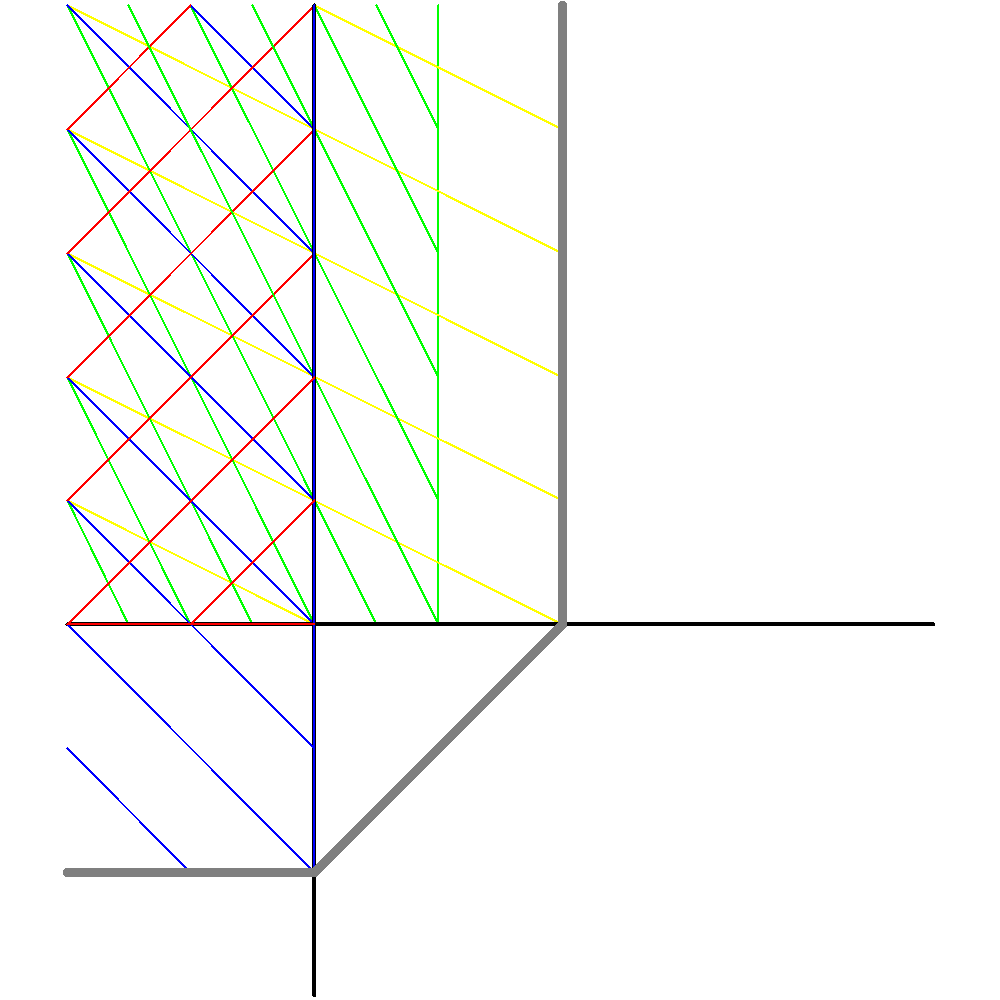
\includegraphics[width=6cm]{beispiele/img/a.png}
\end{center}
also $\slopes(P_a)=\{0\}$ also ist $P_a$ regulär singulär

% vim: set ft=tex :

\subsection{zweites}
\[
  P_b=t\partial_t^2+2\partial_t-1
\]

$
P_b=t\partial_t^2+2\partial_t-1 \Rightarrow 
\begin{cases}
  k=2,l=1 & \Rightarrow u\leq l=2, v\geq l-k=-1\\
  k=1,l=0 & \Rightarrow u\leq 1, v\geq -1\\
  k=0,l=0 & \Rightarrow u\leq 0, v\geq 0\\
\end{cases}
$

\begin{center}
  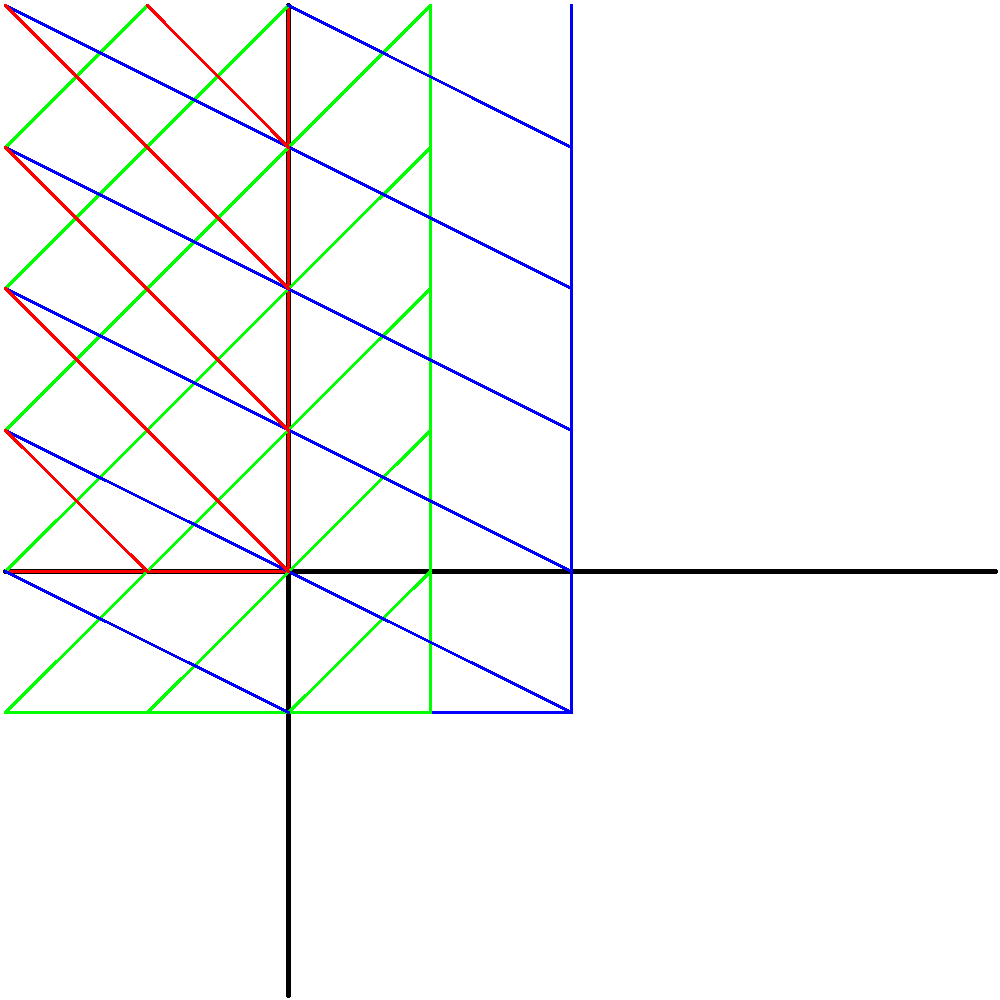
\includegraphics[width=6cm]{beispiele/img/b.png}
\end{center}
also $\slopes(P_b)=\{0\}$ also ist $P_b$ regulär singulär

% vim: set ft=tex :

\subsection{drittes}

\begin{comment}
  zula Barbara Seite 46
\end{comment}


\[
  P_c=t^2\partial_t+1
\]
$
P_c=t^2\partial_t+1
\Rightarrow
\begin{cases}
  k=1, l=2 & \Rightarrow u \leq 1, v \geq 1\\
  k=0, l=1 & \Rightarrow u \leq 0  v \geq 0\\
\end{cases}
$
\begin{center}
  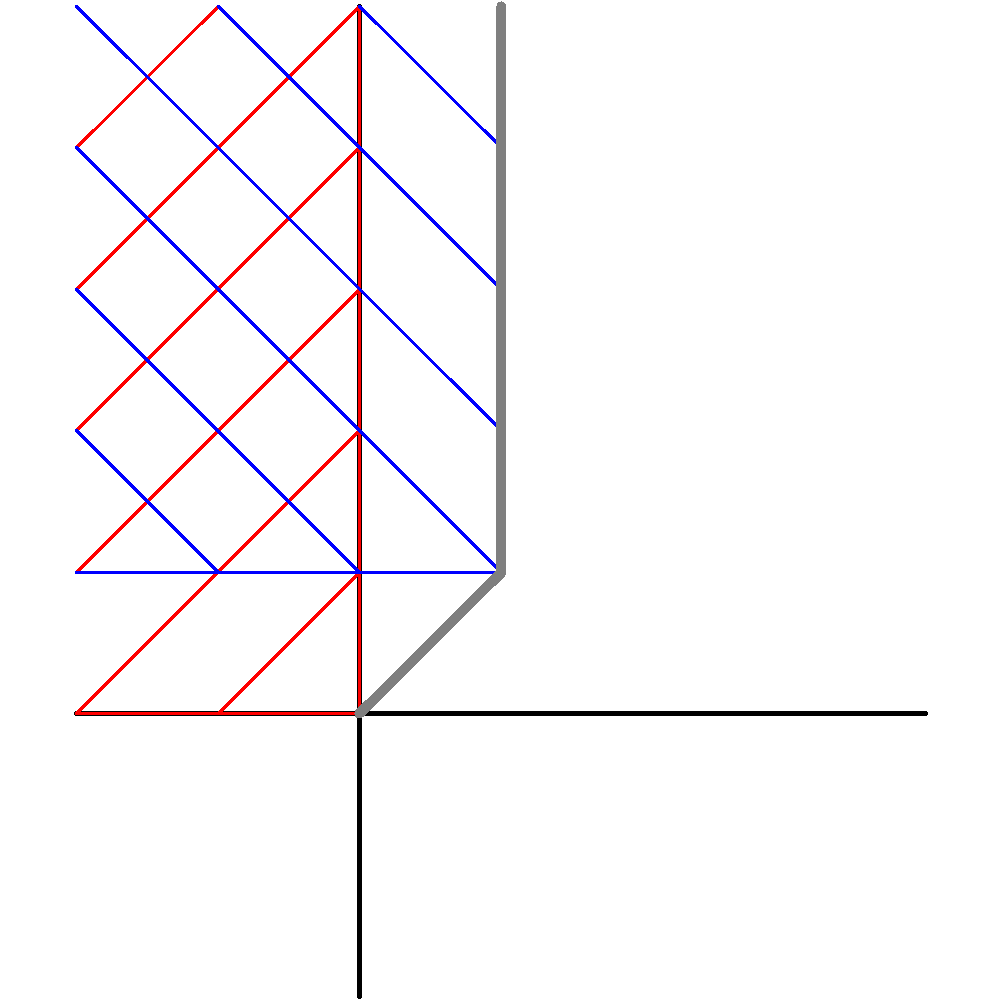
\includegraphics[width=6cm]{beispiele/img/c.png}
\end{center}

also $\slopes(P_c)=\{1\}$.

% vim:set ft=tex :

\subsection{viertes}

\begin{comment}
  zula Barbara Seite 46
\end{comment}

\begin{comment}
  Original aus der Zula:
  \[
    P_d=-3t^{14}\partial_t^6+t^{11}(t+3)\partial_t^5 + 2t^8\partial_t^4
    -t^6(t^3+1)\partial_t^3 + t^4\partial_t
  \]

  $ P_d \Rightarrow
  \begin{cases}
    k=6,l=14 & \Rightarrow u\leq k=6, v\geq l-k=8\\
    k=5,l=12 & \Rightarrow u\leq 5, v\geq 7\\
    k=5,l=11 & \Rightarrow u\leq 5, v\geq 6\\
    k=4,l=8 & \Rightarrow u\leq 4, v\geq 4\\
    k=3,l=9 & \Rightarrow u\leq 3, v\geq 6\\
    k=3,l=6 & \Rightarrow u\leq 3, v\geq 3\\
    k=1,l=4 & \Rightarrow u\leq 1, v\geq 3\\
  \end{cases} $

  also ist Abbildung 5.8 auf seite 53 der zula falsch?
\end{comment}

\[
  P_d=-3t^{14}\partial_t^6+t^{11}(t+3)\partial_t^5 + 2t^8\partial_t^4
  -t^6(t^3+1)\partial_t^3 + t^3\partial_t
\]

$ P_d \Rightarrow
\begin{cases}
  k=6,l=14 & \Rightarrow u\leq k=6, v\geq l-k=8\\
  k=5,l=12 & \Rightarrow u\leq 5, v\geq 7\\
  k=5,l=11 & \Rightarrow u\leq 5, v\geq 6\\
  k=4,l=8 & \Rightarrow u\leq 4, v\geq 4\\
  k=3,l=9 & \Rightarrow u\leq 3, v\geq 6\\
  k=3,l=6 & \Rightarrow u\leq 3, v\geq 3\\
  k=1,l=3 & \Rightarrow u\leq 1, v\geq 2\\
\end{cases} $

\begin{center}
  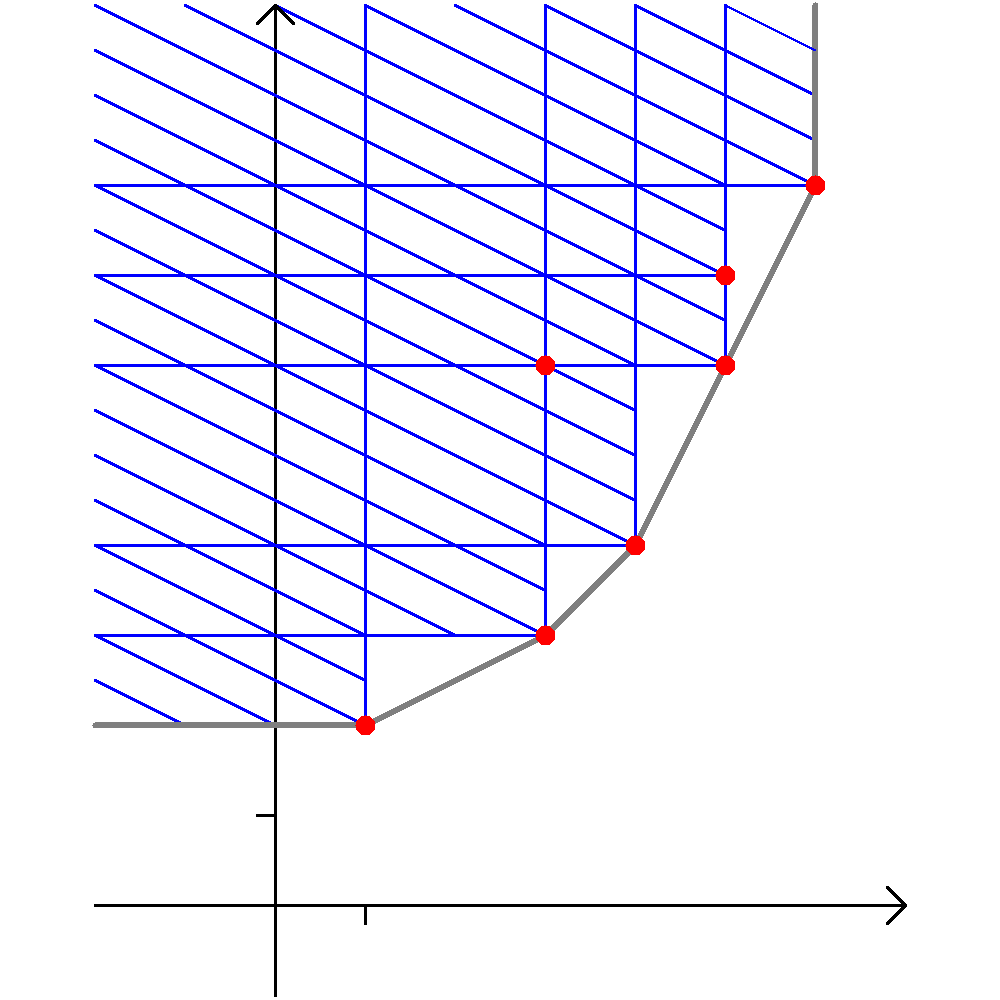
\includegraphics[width=6cm]{beispiele/img/d.png}
\end{center}
also $\slopes(P_b)=\{0,\frac{1}{2},1,2\}$ also ist $P_d$ irregulär singulär.\\
Offenbar ist der Hauptnenner der Steigugnen gleich $2$.\\
Betrachte also $\rho:t\mapsto u^2$\\
und erhalte: ???

% vim: set ft=tex :

\subsection{bsp e}

\[
  P_e=t^4(t+1)\partial_t^4 + t\partial_t^2+\frac{1}{t}\partial_t+1
\]

\begin{center}
  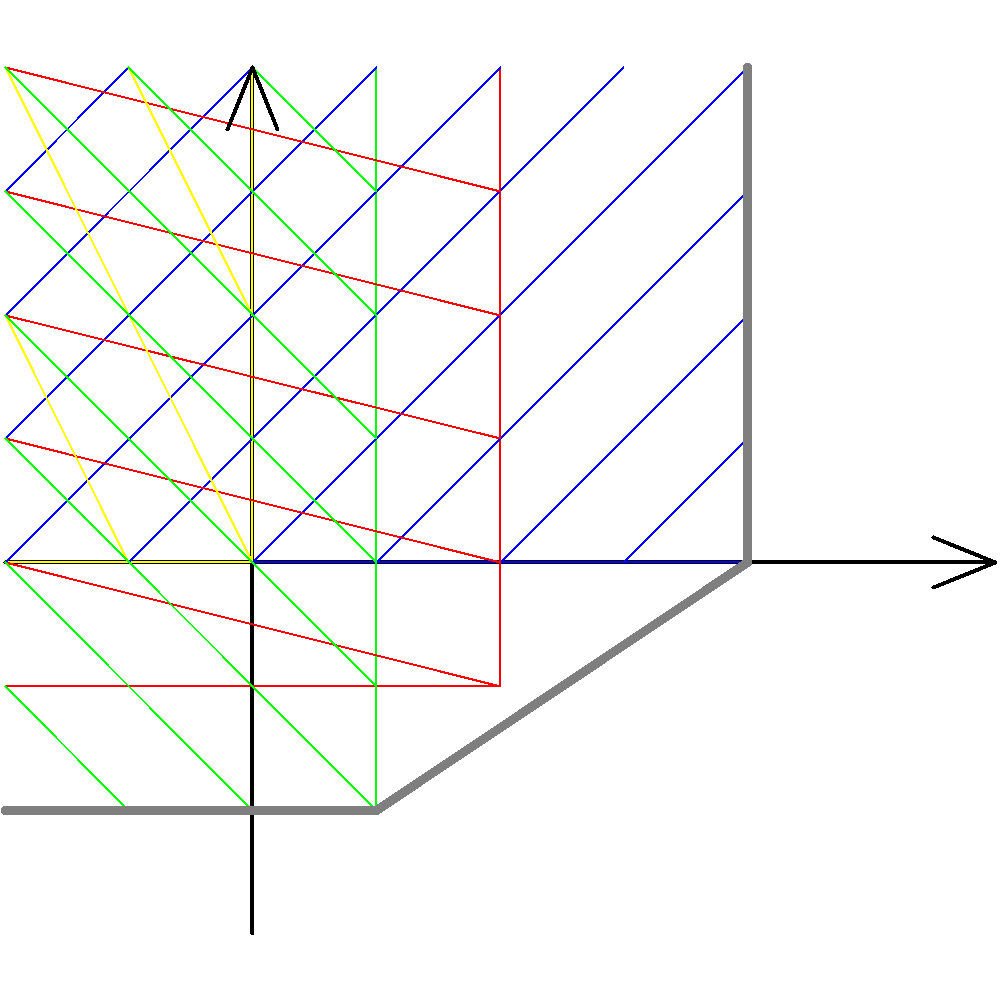
\includegraphics[width=6cm]{beispiele/img/e.png}
\end{center}

also $\slopes(P_e)=\{0,\frac{2}{3}\}$

Dies gilt Analog für das einfachere:
\[
  \bar P_e=t^4\partial_t^4 +\frac{1}{t}\partial_t
\]

\begin{center}
  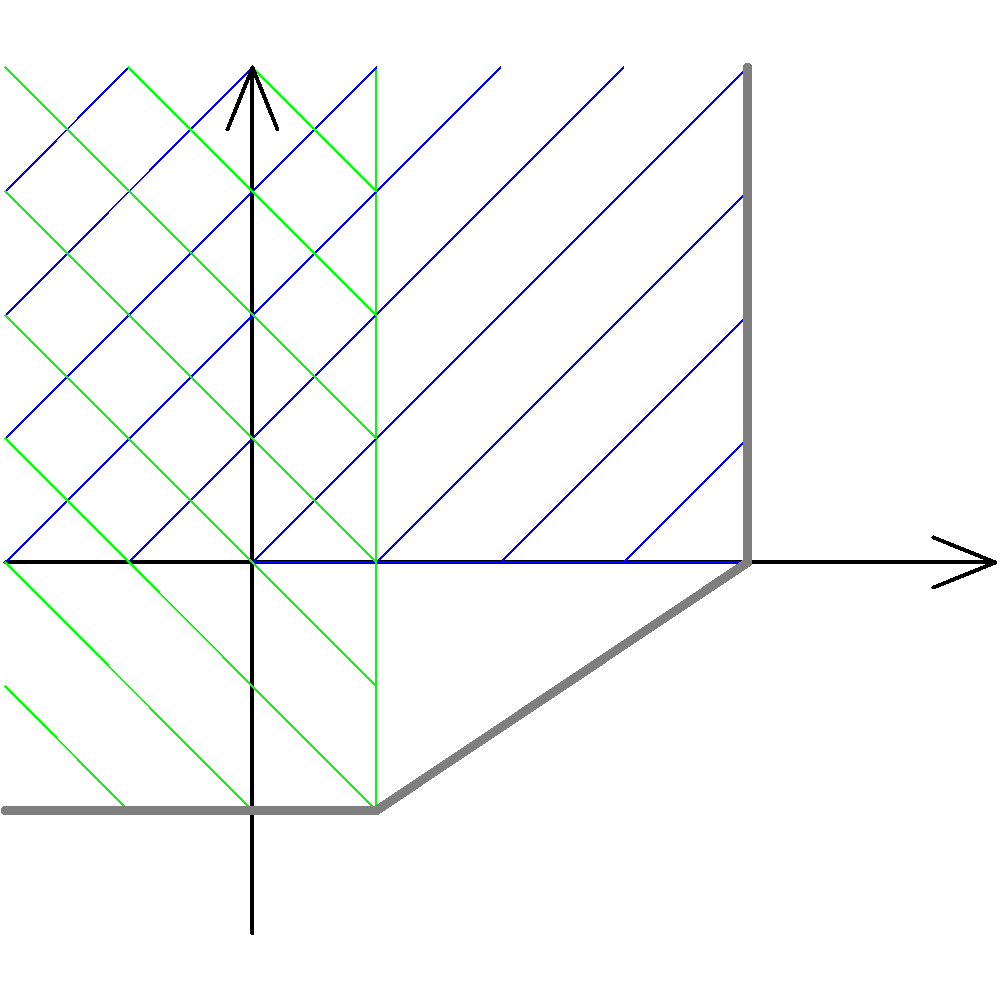
\includegraphics[width=6cm]{beispiele/img/bar_e.png}
\end{center}

% vim: set ft=tex :

\begin{comment}
  \[
    Sabbah\_Fourier-local.pdf \rightarrow 5.b.
  \]
\end{comment}
\section{Meromorpher Zusammenhang der formal, aber nicht Konvergent, zuerfällt}
\begin{comment}
  Quellen??
  \[
    \sum n!x^n
  \]
\end{comment}

% vim: set ft=tex :


%%%%%%%%%%%%%%%%%%%%%%%%%%%%%%%%%%%%%%%%%%%%%%%%%%%%%%%%%%%%%%%%%%%%%
\appendix
\addcontentsline{toc}{chapter}{Anhang}

\begin{landscape}
  %\chapter{zur aufteilung in Lemma 2.4}
  \chapter{Aufteilung von ...}
  \label{chap:aufteilung}
  Sei $\phi\in u^{-1}\C[u^{-1}]$, so ist $\phi'=:\sum_{i=2}^N a_{-i}u^{-i}\in u^{-2}\C[u^{-1}]$ also 
  $u\phi'(u)=\sum_{i=1}^N a_{-i-1}u^{-i} \in u^{-1}\C[u^{-1}]$, welches wir zerlegen wollen.\\
  Zerlege also $u\phi'(u)=\sum_{j=0}^{p-1}u^j\psi_j(u^p)$
  mit $\psi_j\in\C[t^{-1}]$ für alle $j>0$ und $\psi_0\in
  t^{-1}\C[t^{-1}]$:\\
  \begin{center}
    \begin{tikzpicture} [descr/.style={fill=white,inner sep=2.5pt}]
    \matrix (m) [
      matrix of math nodes,
      row sep=1em,
      %column sep=-0.7em,
      text height=1.5ex,
      text depth=0.25ex]
    {
      & & & & & & & & & & & & & & \, \\
      u\phi'(u)= &
      a_{-2}u^{-1} &
      +...+ &
      a_{-p}u^{-(p-1)} &
      + &
      a_{-(p+1)}u^{-p} &
      + &
      a_{-(p+2)}u^{-(p+1)} &
      +...+ &
      a_{-2p}u^{-(2p-1)} &
      + &
      a_{-(2p+1)}u^{-2p} &
      + &
      a_{-(2p+3)}u^{-(2p+1)} &
      + ...  \\
      & & & & & & & & & & & & & & \, \\
    };

      \path[solid]
      (m-2-6) edge [bend left=20] node[descr]{$\psi_0(u^p)$} (m-2-12)
      (m-2-12)  edge [bend left=20] (m-1-15);

      \path[dotted]
      (m-2-4) edge [bend right=20] node[descr]{$u\psi_1(u^p)$} (m-2-10)
      (m-2-10)  edge [bend right=20] (m-3-15);

      \path[dashed]
      (m-2-2) edge [bend right=20] node[descr]{$u^{p-1}\psi_{p-1}(u^{p})$} (m-2-8)
      (m-2-8) edge [bend right=20] (m-2-14)
      (m-2-14) edge [bend right=20] (m-3-15);
    \end{tikzpicture}
  \end{center}
  also:\\
  \begin{eqnarray*}
    \psi_0(u^p) & = & a_{-(p+1)}u^{-p}+a_{-(2p+1)}u^{-2p}+...\\
    \psi_1(u^p) & = & a_{-p}u^{-p}+a_{-2p}u^{2p}+...\\
    & \vdots & \\
    \psi_{p-1}(u^p) & = & a_{-2}u^p+a_{-(p+2)}u^{2p}+...\\
  \end{eqnarray*}
\end{landscape}


\nocite{*}
%\bibliographystyle{dinat}
\bibliographystyle{plain}
\bibliography{main}

\end{document}
